\section*{Appendix B}
\addcontentsline{toc}{section}{\numberline{}Appendix B}
%\appendix
%\section{Príloha}
\subsection*{User manual}
MathworldVR user manual gives an assistance to people using it. It includes described images of VR headset, controllers usage and screenshots of virtual user interface.

\subsubsection*{HTC Vive headset}
\begin{figure}[ht!]
\centering
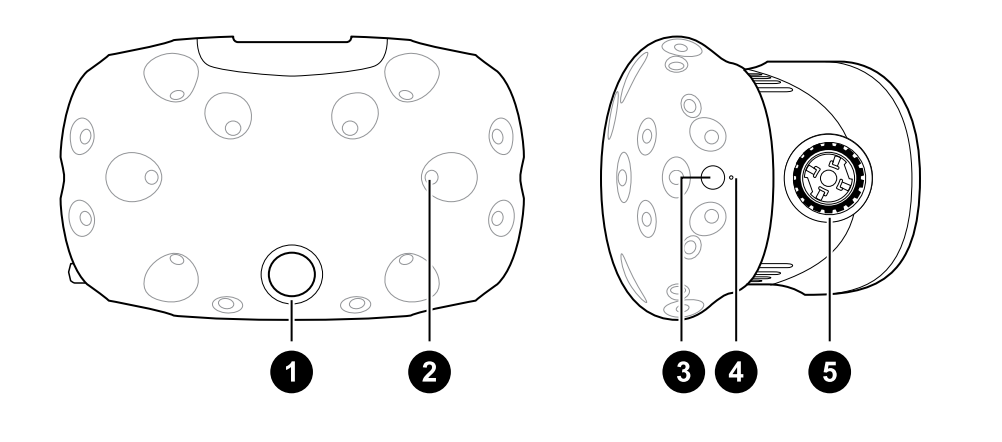
\includegraphics[width=0.8\textwidth]{htc-vive-headset.png}
\caption{HTC Vive headset - technical detail. \cite{htc-vive-user-guide}}
\label{r:75}
\end{figure}

\begin{enumerate}
\item{Camera lens - can be used for viewing the "real world" from within the headset.}
\item{Tracking sensor - allowing Lighthouse base stations to "see" the headset.}
\item{Headset button - used for opening the SteamVR menu from within virtual reality view.}
\item{Status light - if the light produces red color, headset is not ready; if the light produces green color, headset is ready to be used.}
\item{Lens distance knob - used for changing the distance between lenses.}
\end{enumerate}

\newpage
\subsubsection*{Hand controllers}
\begin{figure}[ht!]
\centering
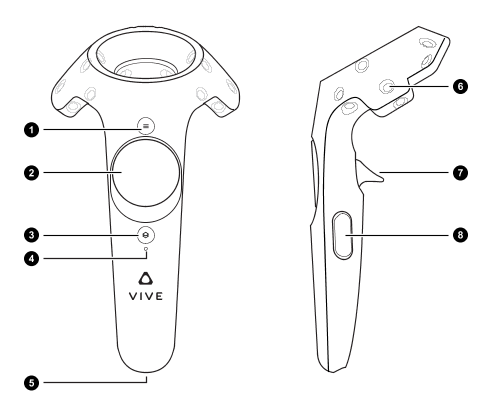
\includegraphics[width=0.9\textwidth]{vive-controllers.png}
\caption{HTC Vive hand controllers - technical detail. \cite{htc-vive-user-guide}}
\label{r:76}
\end{figure}

\begin{enumerate}
\item{Menu button - This button doesn't have any effect in MathworldVR.}
\item{Trackpad - Allows user to move in scrolling menus, just like double-finger gesture on notebook trackpads. It's also clickable. Clicking and holding the trackpad on the left controller will trigger teleportation beam. User can point the beam where he wants to be teleported and then release the trackpad.}
\item{System button - Used for opening the SteamVR menu.}
\item{Status light - Indicates the status of a controller. Green color means it's ready, blinking orange color means it needs to be recharged and blue color means it needs to be synced with the Lighthouse base stations, because they cannot see the controller.}
\item{Micro-USB port - Used for recharging the controller and also to upgrade its firmware.}
\item{Tracking sensor - Thanks to this sensor, Lighthouse base stations can see the controller. Tracking of HTC Vive controllers is very precise, because Lighthouse base stations emits laser beam that maps the space in front of them.}
\item{Trigger button - Used for selecting the options and moving the sliders in SettingsPanel component.}
\item{Grip button - Used for grabbing and scaling the parmetrized function. For grabbing interaction, only one of two controller's grip buttons needs to be pressed. For scaling interaction, both left and right controller's grip buttons needs to be pressed, scaling the grabbed object up and down according to movement of both controllers.}
\end{enumerate}

\newpage
\subsubsection*{Interacting with parametrized function}
Parametrized function can be grabbed, scaled and its variables changed in settings panel. To grab the function, you need to press the grip button on one of your VR controllers. You can move and rotate the function freely while grabbing it, just like objects in real life. To scale the function, you need to press grip buttons on both VR controllers imultaneously and move them fro or to each other. Moving controllers to each other will make the function smaller. Moving controllers from each other will make the function bigger.

\begin{figure}[ht!]
\centering
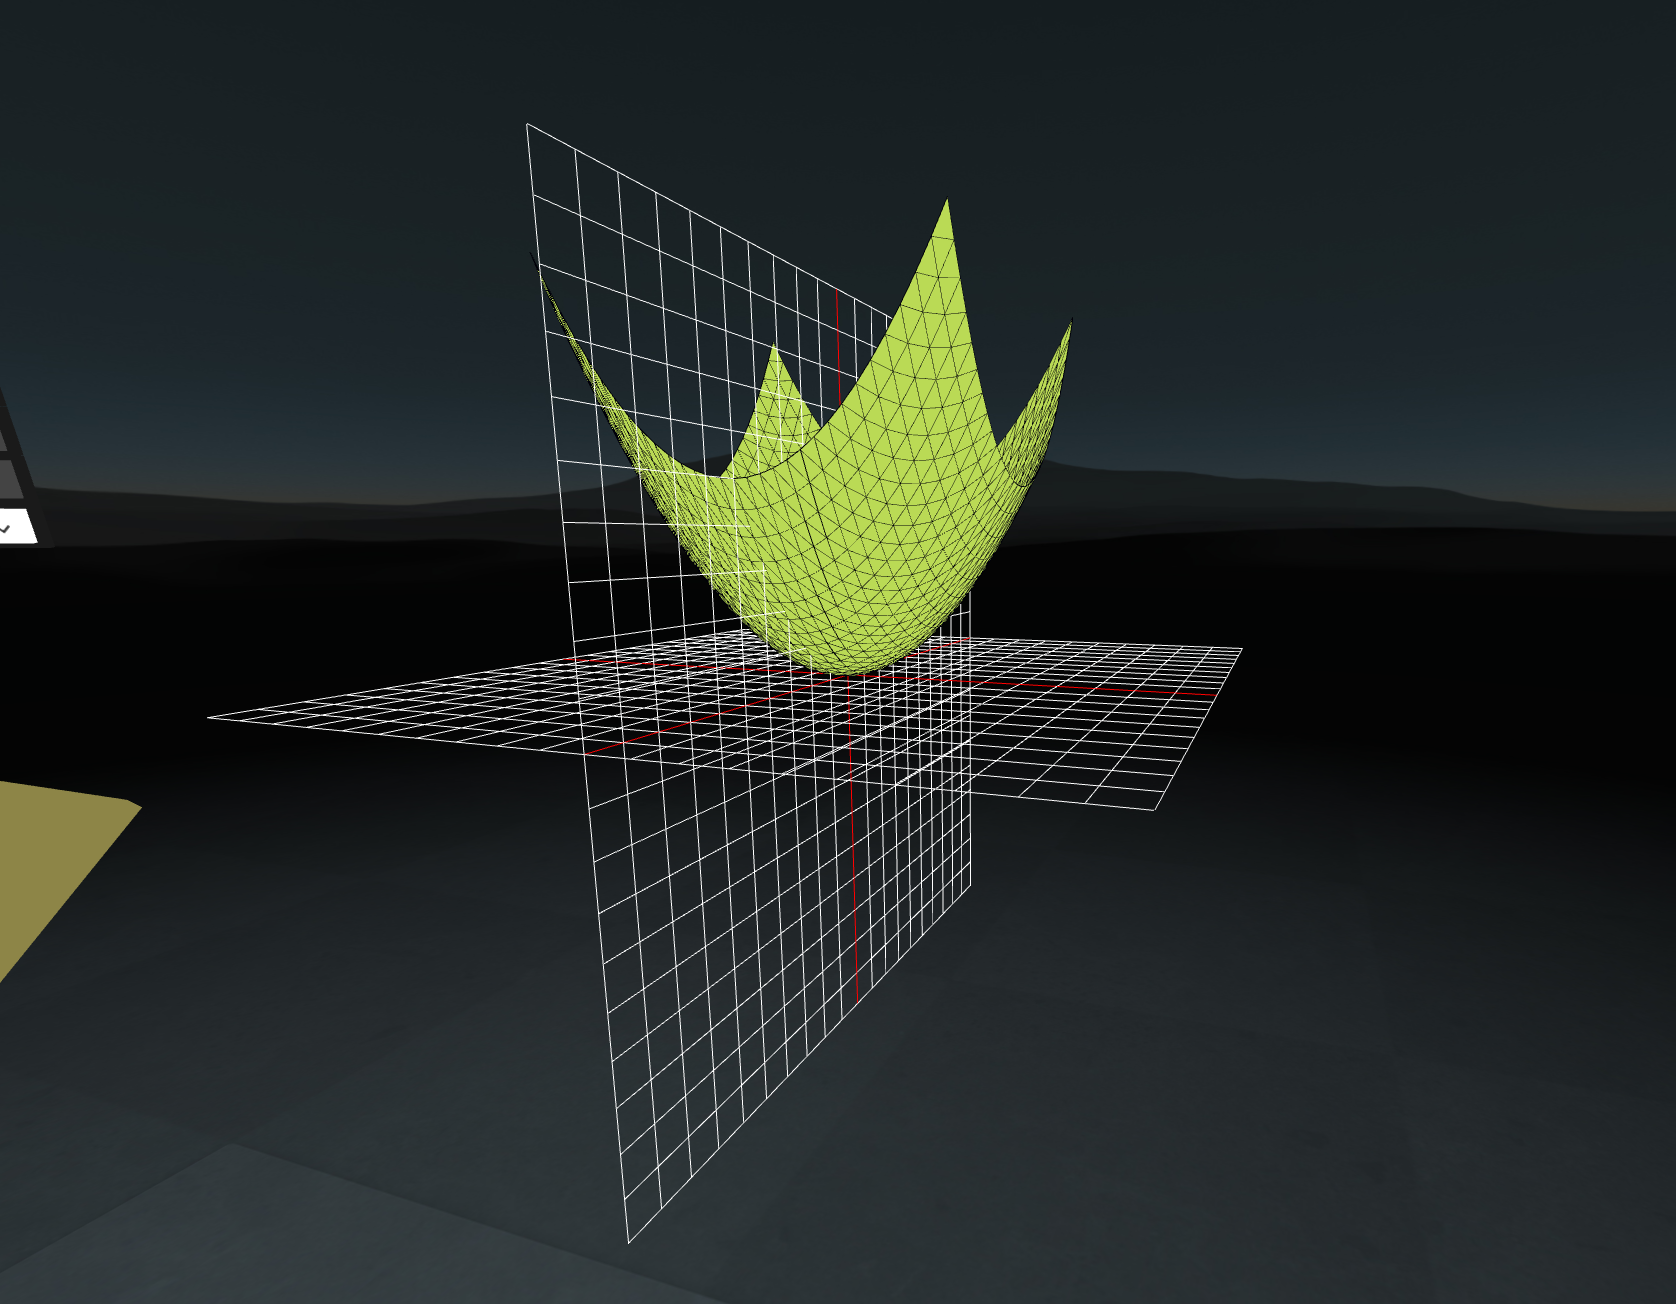
\includegraphics[width=0.9\textwidth]{pfunc-component.png}
\caption{ParametrizedFunction component.}
\label{r:77}
\end{figure}

\newpage
\subsubsection*{Changing function variables and color}
To change the function variables or its color, you can use the SettingsPanel component. Pointing the VR controller at this panel will initiate the laser pointer. Move the pointer at any slider and press the trigger button. Holding and moving the controller will change the value of selected variable. You can also press and hold the grip button while pointing at SettingsPanel - this will automatically move the panel on top of your controller.
 
\begin{figure}[ht!]
\centering
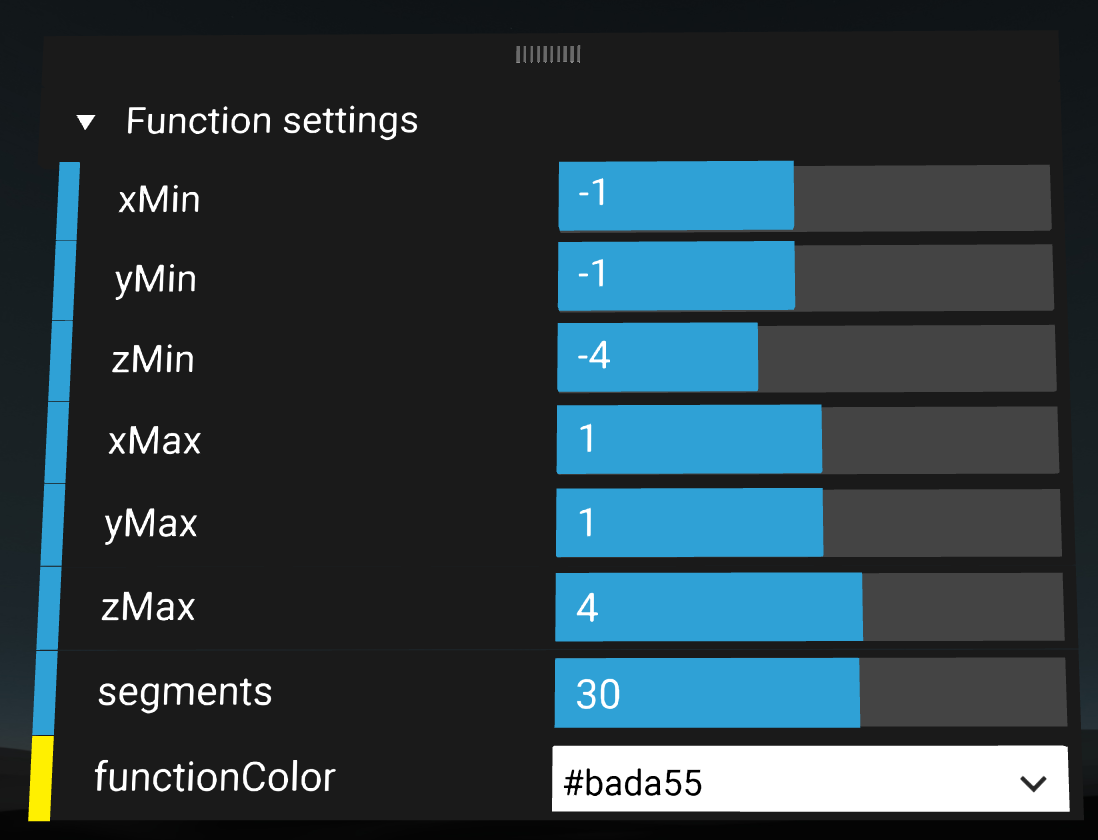
\includegraphics[width=0.9\textwidth]{settings-component.png}
\caption{Settings component.}
\label{r:78}
\end{figure}

\newpage
\subsubsection*{User input}
You can change right side of the equation by simply clicking the buttons on virtual calculator. This component was designed to resemble real calculator and make user interaction with it more intuitive. After you write the function, you can update the 3D visualization by clicking the \textsl{Update} button on virtual calculator.

\begin{figure}[ht!]
\centering
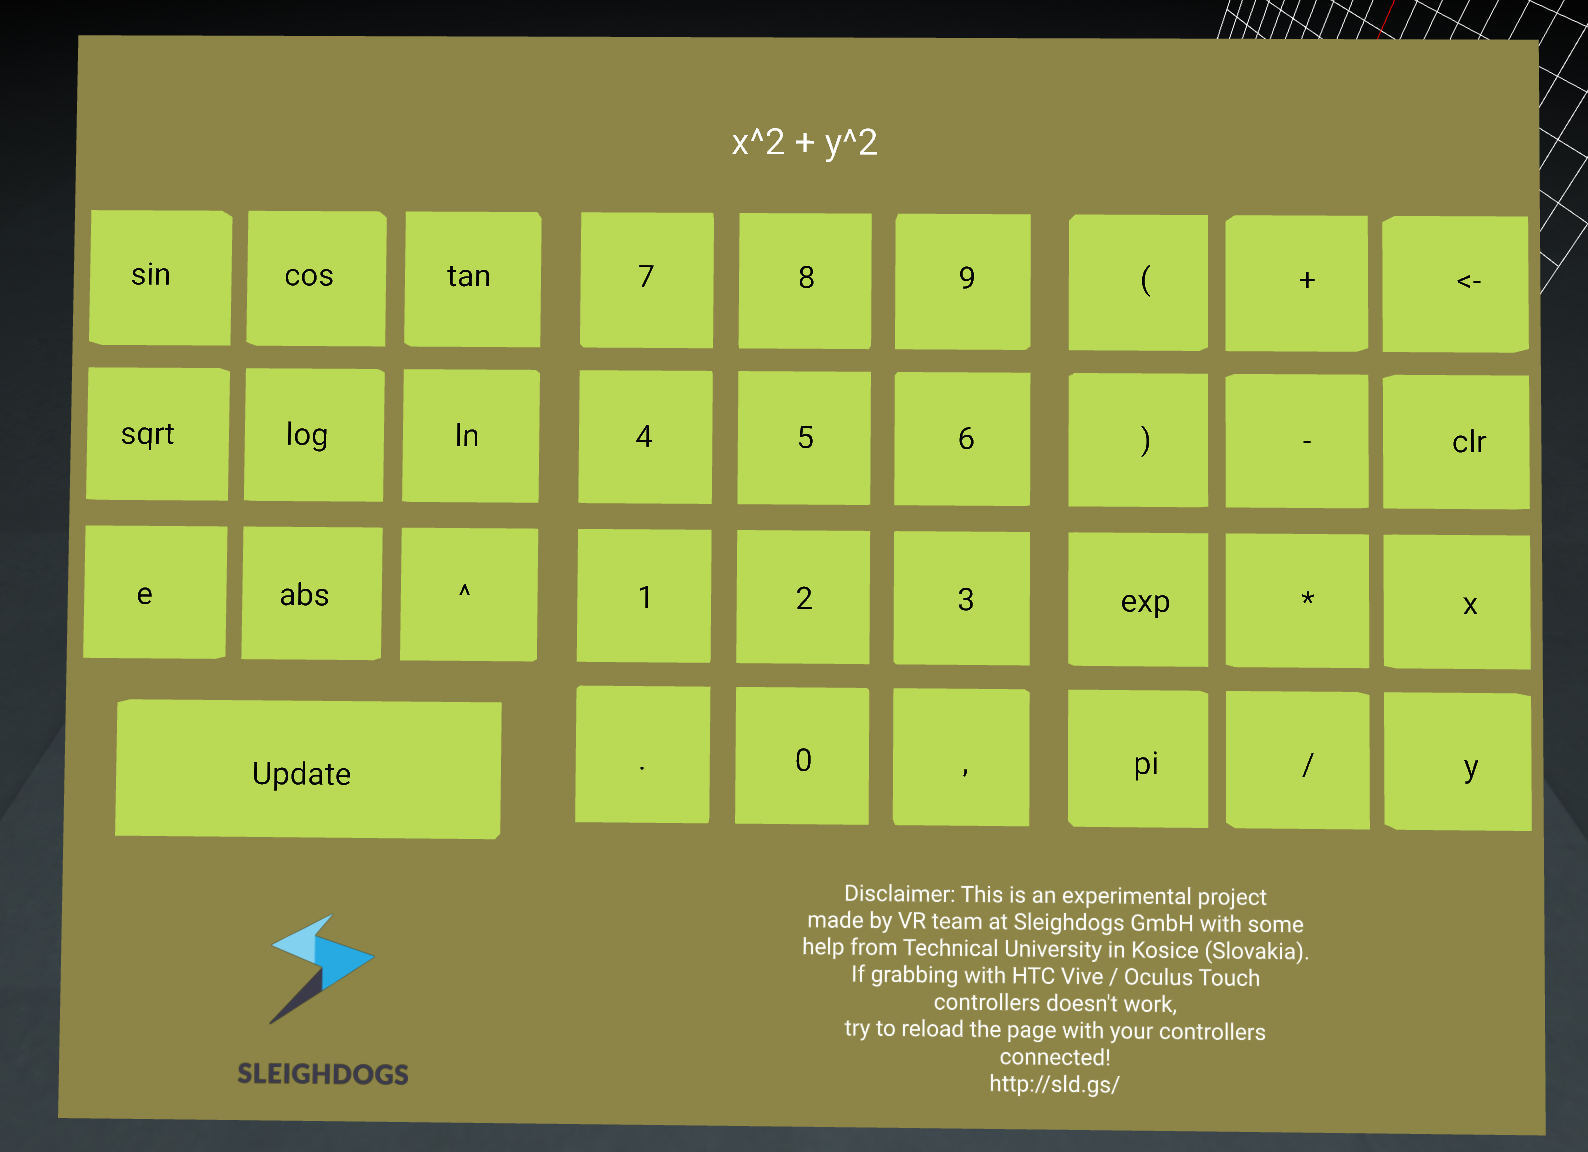
\includegraphics[width=0.9\textwidth]{calculator-component.png}
\caption{Calculator component.}
\label{r:78}
\end{figure}